\documentclass{article}
\usepackage{graphicx}
\usepackage{float}
\usepackage{amsmath}
\graphicspath{{images/}}
\usepackage{caption}
\captionsetup[figure]{position = below,}
\usepackage{listings}
\usepackage{xcolor}
\usepackage{amssymb}
 \usepackage{amsthm}
 \usepackage{amsfonts}
\usepackage{braket}
\DeclareCaptionFont{white}{\color{white}}
\DeclareCaptionFormat{listing}{%
\parbox{\textwidth}{\colorbox{gray}{\parbox{\textwidth}{#1#2#3}}\vskip-4pt}}
\captionsetup[lstlisting]{format=listing,labelfont=white,textfont=white}
\lstset{frame=lrb,xleftmargin=\fboxsep,xrightmargin=-\fboxsep, columns=fullflexible}

\title{\textbf{Deutsch-Jozsa Algorithm}}

\author{Indranil Ghosh\\Jadavpur University, Physics Department\\ UG-III\\ Email: indranilg49@gmail.com}

\date{\today}

\begin{document}
\maketitle

\begin{abstract}
This project is to compare the simulation of Deutsch-Jozsa Algorithm, between IBM's Quantum Experience's real quantum simulator and a  Python program that  has been designed, available in Github (https://github.com/indrag49/Quantum-SimuPy), for  simulating the ideal case. Packages used: Numpy, Pandas and Mathplotlib. The quantum gates and the functions required for this simulation are available in the program and can be easily implemented. The moto of this project is to use python packages to design a quantum simulator for performing simple quantum computations.
\end{abstract}

\section{Introduction}
The \textit{Deutsch-Jozsa Algorithm}, a quantum algorithm, was devised by David Deutsch and Richard Jozsa in the year 1992, which was later improved by \textit{Cleve et al. in 1998}. This is a more general quantum algorithm derived from \textit{Deutsch Algorithm} which was developed by David Deutsch in 1985 and was non-deterministic in nature. DJ Algorithm is rather deterministic in nature and served as the first algorithm that raised a barrier between the classical and quantum difficulty of a problem.

\section{The Problem}
Suppose there are two participants: a sender(\textbf{S}) and a reciever(\textbf{R}) situated at a large distance from one another. \textbf{S} tends to send a number $x$, between $0$ and $2^n - 1$ to \textbf{R}. \textbf{R} has a quantum black box operator, the \textit{oracle} that implements the function $f(x)$, which takes n-digit binary values as inputs and outputs either $0$ or $1$ for each such values, i.e, $f: [0, 1]^n \rightarrow [0, 1]$. Now, it is sure that, $f(x)$ is only of two kinds,
\begin{center}
1. Constant, for all values of x, or \\ \par
2. Balanced, i.e, is equal to $1$ for exactly half of all the possible $x$s and $0$ for the other half.
\end{center} 
The algorithm determines with certainty whether$f$ used is Constant or Balanced by using the oracle $U_f$. In the originial non-determinstic algorithm by Deutsch, the function $f$ had 1 bit as input and the goal was to determine whether $f$ was constant. $f:[0, 1] \rightarrow [0, 1]$. A deterministic algorithm is a type of algorithm which always outputs the same result for a particular input.
\section{The Classical counterpart}
Classically, \textbf{S} needs to know from \textbf{R} $2^{n-1} + 1$ times, in the worst case scenario. This can be viewed in the following way: Let \textbf{S} gets signal everytime from \textbf{R} after \textbf{R} implements the function $f$ using the oracle. \textbf{S} needs to recieve $2^{n-1}$ $0$s before getting a $1$ or a $0$, which determines whether $f$ is balanced or constant. so, the best classical algorithm needs $2^{n-1} + 1$ signals to be received before determining the kind of $f$. But using the DJ algorithm this is possible by only one function implementation. Classically, the best case occurs where the function is balanced and the first two signals are different, verifying the nature of $f$.

\section{Action of the Oracle}
The action of the \textit{Oracle} can be depicted as, 
\begin{center}
$U_f \ket{x} \ket{q} = \ket{x} \ket{q \bigoplus f(x)}$
\end{center}
Here, $\ket{x}$ is the index register, $\bigoplus$ denotes addition modulo $2$ and the oracle qubit $\ket{q}$, a single qubit which flips if $f(x)=1$ and else remains unchanged. 

\section{Algorithm Procedure}
\begin{figure}[H]
\centering 
\noindent\makebox[\textwidth]{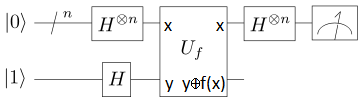
\includegraphics[scale=0.6]{DJ7}}%
\caption{Deutsch-Jozsa Algorithm Circuit [Figure from Wikipedia]}
\end{figure}
Initially, to start with, the Sender, \textbf{S} has an $n$ qubit register, \textbf{r}, to send the number $x$ to the Receiver, \textbf{R},  and a single qubit register to store the signal  \textbf{R} sends, by using quantum parallelism and evaluating $f$.  That is, the initial state, let be depicted by $\ket{P}$, be $\ket{0}^{ \otimes n} \ket{1}$. $\ket{P}=\ket{0}^{ \otimes n} \ket{1}$. Applying Hadamard transform to each registers, we get the qubit state, 
\begin{center}
$\ket{P2}={1 \over \sqrt{2^n}}\sum_{x=0}^{2^n-1}{\ket{x}{(\ket{0}-\ket{1}) \over \sqrt{2}}}$.
\end{center}
Next, \textbf{R} evaluates $f$ by applying the quantum oracle matrix $U_f$ to $\ket{P}$,
\begin{center}
$\ket{P3}=U_f\ket{P2}={1 \over \sqrt{2^n}}\sum_{x=0}^{2^n-1}{\ket{x}{(\ket{f(x)} - \ket{1 \oplus f(x)}) \over \sqrt{2}}}={1 \over \sqrt{2^n}}\sum_{x=0}^{2^n-1}{(-1)^{f(x}\ket{x}{(\ket{0} - \ket{1}) \over \sqrt{2}}}$
\end{center}
For each $x$, $f(x)$ is either $0$ or $1$.  \textbf{S} now possesses an array of qubits in which the evaluation of $f$ is stored. At the next step, the last qubit, the signal register, is ignored as \textbf{S} interferes terms in the superposition using Hadamard transform on \textbf{r}. Our work now is to define the effect of Hadamard transform on a state $\ket{x}$.
\begin{center}
${H^{\otimes n}\ket{x_0, x_1,...,x_{n-1}}} = {\sum_{y_0, y_1,...,y_{n-1}}(-1)^{x_0 y_0 \oplus x_1 y_1 \oplus...\oplus x_{n-1}y_{n-1}}\ket{y_0,y_1,...,y_{n-1}}\over \sqrt{2^n}}$\\ \par
$\Rightarrow H^{\otimes n}\ket{x}={\sum_{y} (-1)^{x.y}\ket{y} \over \sqrt{2^n}}$
\end{center}
Here, $x.y$ is the sum of the bitwise inner product of $x$ and $y$ modulo $2$. Evaluating the final state we get, 
\begin{center}
${1\over {2^n}}\sum_{x=0}^{2^n-1} \sum_{y=0}^{2^n-1} (-1)^{x.y+f(x)}\ket{y}{(\ket{0}-\ket{1})\over \sqrt{2}}$
\end{center}
The probability of measuring $\ket{0}^{\otimes n}$ is ,
\begin{center}
$|{1\over {2^n}}\sum_{x=0}^{2^n-1} (-1)^{f(x)}|^2$
\end{center}
So, now we can determine $f(x)$ by running the experience once.\\  
1. Probability is $1$ if $f(x)$=constant i.e., constructive interference\\ 
2. Probability is $0$ if $f(x)$=balanced i.e., destructive interference  [All the terms in the sum over $x$ cancel each other]
\subsection{Steps}
1. Initialise $n+1$ qubits with $n$ qubits in all zero states, $\ket{00...0}$ and the last qubit in one state, $\ket{1}$.\\ 
2. Apply Hadamard Transform to each qubits.\\ 
3. Apply the Oracle matrix $U_f$ to the current superposition state.\\ 
4. Neglect the last qubit and apply Hadamard Transform again to the remaining qubits.\\ 
5. Perform measurement on each qubit.\\ 

\section{Comparison Of The Example Circuits}
We consider $n=3$ and $f(x)=x_0 \oplus x_1x_2$. This function is balanced as flipping the bit $x_0$ flips the value of $f(x)$ irresepective of $x1$ and $x2$.
\subsection{IBM Q Experience Results}
\begin{figure}[H]
\centering 
\noindent\makebox[\textwidth]{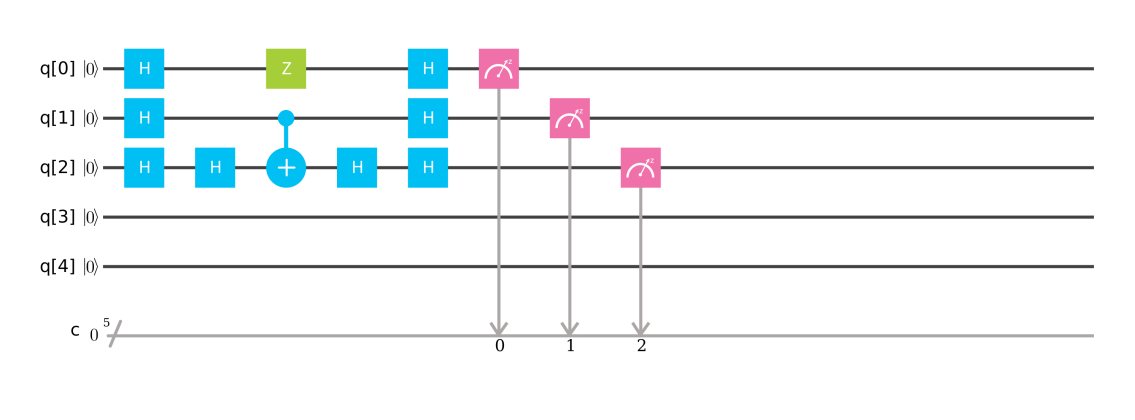
\includegraphics[scale=0.3]{DJ1}}%
\caption{Algorithm Circuit[Figure from IBM Q experience’s home page]}
\end{figure}
\begin{figure}[H]
\centering 
\noindent\makebox[\textwidth]{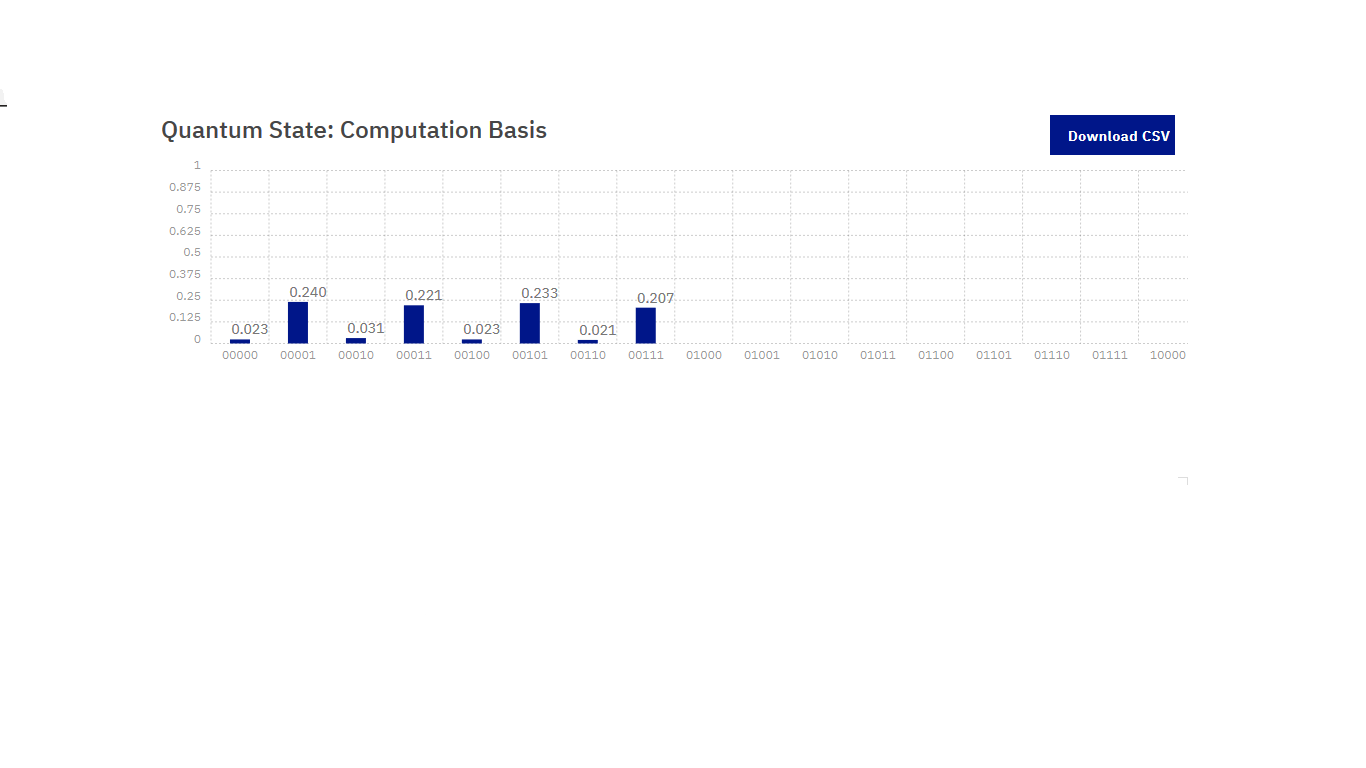
\includegraphics[scale=0.4]{DJ2}}%
\caption{Probability Distribution, with noise[Figure from IBM Q experience’s home page]}
\end{figure}
\subsection{Python Simulation}
\begin{lstlisting}[language=Python, frame=single]
k=np.kron
H=Hadamard(I2)
Z=PauliZ(I2)
cnot=CNOT(I4)
h=k(k(H, H), H)
h1=k(I2, H)
U_f=k(Z, h1.dot(cnot.dot(h1)))
m=h.dot(U_f.dot(h.dot(Q000)))
p=measure(m)
print(p)
plot_measure(p)
\end{lstlisting}
\begin{figure}[H]
\centering 
\noindent\makebox[\textwidth]{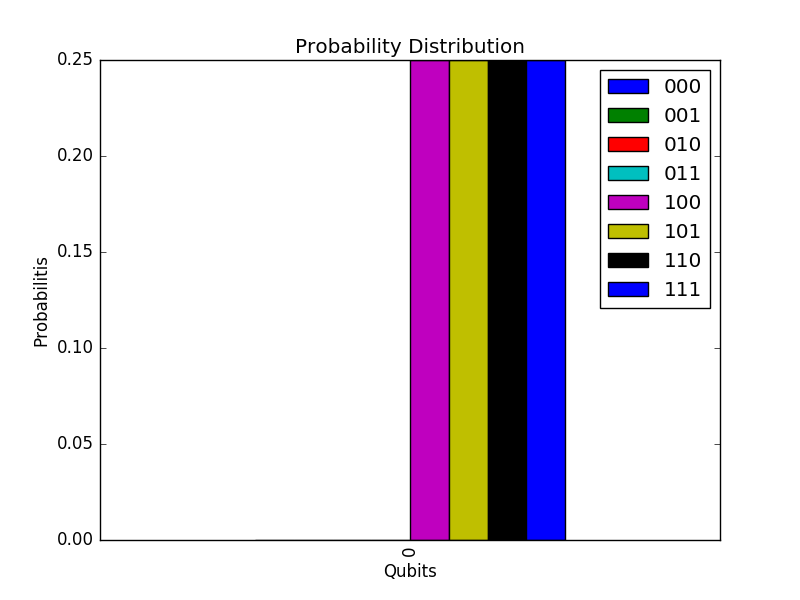
\includegraphics[scale=0.4]{DJ3}}%
\caption{Probability Distribution, without noise}
\end{figure}
For constant $f(x)$,
\subsection{IBM Q Experience Results}
\begin{figure}[H]
\centering 
\noindent\makebox[\textwidth]{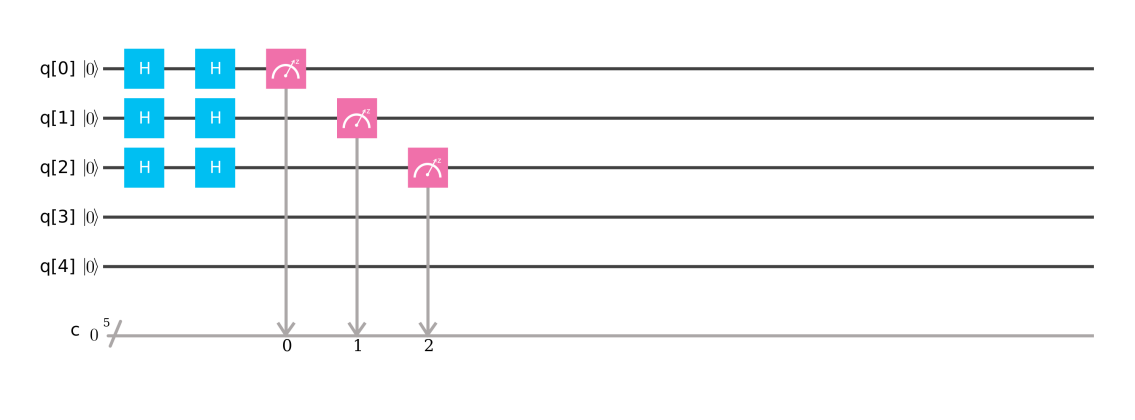
\includegraphics[scale=0.3]{DJ4}}%
\caption{Algorithm Circuit[Figure from IBM Q experience’s home page]}
\end{figure}
\begin{figure}[H]
\centering 
\noindent\makebox[\textwidth]{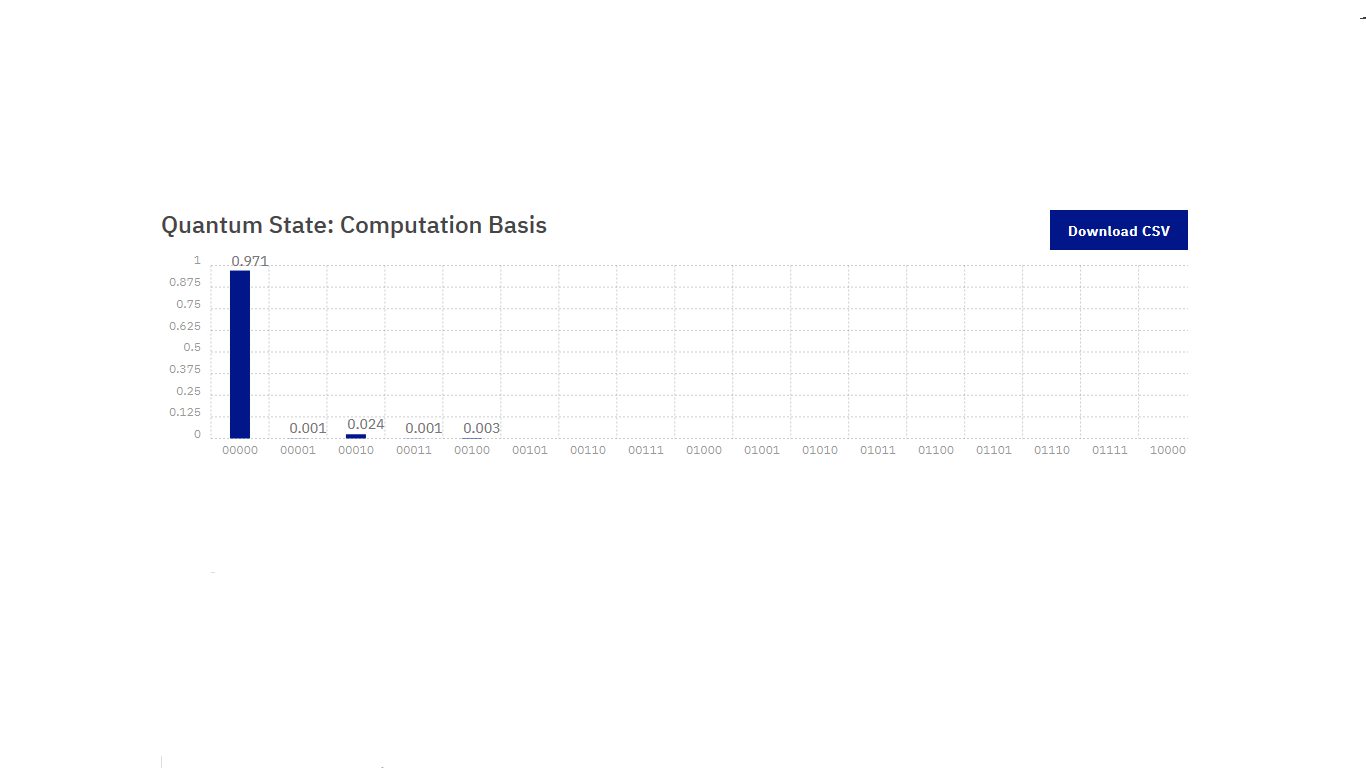
\includegraphics[scale=0.4]{DJ5}}%
\caption{Probability Distribution, with noise[Figure from IBM Q experience’s home page]}
\end{figure}
\subsection{Python Simulation}
\begin{lstlisting}[language=Python, frame=single]
k=np.kron
H=Hadamard(I2)
h=k(k(H, H), H)
m=h.dot(h.dot(Q000))
p=measure(m)
print(p)
plot_measure(p)
\end{lstlisting}
\begin{figure}[H]
\centering 
\noindent\makebox[\textwidth]{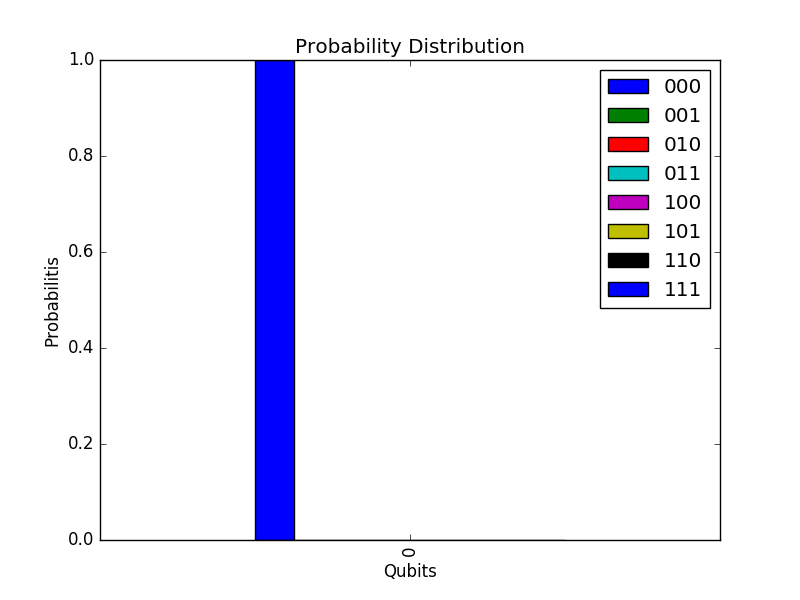
\includegraphics[scale=0.4]{DJ6}}%
\caption{Probability Distribution, without noise}
\end{figure}
\begin{thebibliography}{9}
\bibitem{knuthwebsite}
\texttt{Quantum Computation and Quantum Information by Michael A. Nielsen and Isaac L. Chuang, URL:http://www-reynal.ensea.fr/docs/iq/QC10th.pdf}
\bibitem{knuthwebsite}
\texttt{Wikipedia,Deutsch Jozsa Algorithm, https://en.wikipedia.org/wiki/Deutsch–Jozsa algorithm}
\bibitem{knuthwebsite}
\texttt{IBM Quantum Experience Home Page, https://quantumexperience.ng.bluemix.net/qx/experience}
\bibitem{knuthwebsite}
\texttt{https://github.com/indrag49/Quantum-SimuPy}
\end{thebibliography}
\end{document}

